\section{Git operations}
In this section we explore some of the git operations. We try to do
so, in a different way, if comparing with other manuals. Normally the
manuals we see around just explain how to perform an operation. We
try to go further, so in this manual, we have divided our operations in
three parts. In the first part, we give a description about the
operation. In the second part, we give the pre-conditions, or in other
words, we explain in which conditions the operations can be performed.
Finally, in the last part of each operation, we show what is the
result of perform such operation.

\subsection{Add and Remove}
The operations add and remove are used to add and remove content from
index. As we have said before the index contains all the files and
contents to be added on the next commit.\\

\emph{Git} add does not refer directly to the file. Instead it is like
a map from file to content. If we have a file on the index and we
modify it on the working directory, for this modification to be visible
on the next commit, the file has to be added again to the index.\\

The remove operation removes a file from index, so it will not be
present if we perform a commit exactly after the remove. The removed
file besides of being removed from index, it will also be removed from the 
working directory (if it is still exists there).

\subsubsection{Pre requisites}
The add operation has only one pre-condition. The file has to be in
the working directory. It means that a file that is
on the working directory, can be always added to index.

Relatively to the remove operation there are a few conditions that
have to be satisfied for the remove operation be performed, which are: 
\begin{itemize}
\item The file that is being removed is currently in index;
\item The file that is being removed is in the previous commit, exactly with the same
content.
\end{itemize}

The first restriction is quite obvious. It is not possible to remove
a file if it does not exists. The last restriction exists, to avoid
the accidental deletion of file's contents. It is possible to have a
file in index with a certain content that does not exists in the
repository and since the remove operation removes the file from the index
and from the working directory, the content would be lost.  

\subsubsection{Result}
After performing the add operation there is something that will be
always observed. The file will be in index. Besides, if the file was
marked as not merged then the mark goes away. More details about
merged and unmerged files will be given later.\\

The result from performing the remove operation is that the file is
not anymore in the index. Also here the file will not be marked as
unmerged anymore.

\subsubsection{Examples}

The figure \ref{fig:add1}, shows a simple case of adding a file to the 
index. It can be seen, that no changes are made in the repository nor in the working
directory. The only effect is that the index will contain the new
file.\\

\begin{figure}[tp]
   \begin{minipage}[b]{0.5\linewidth}
      \centering
      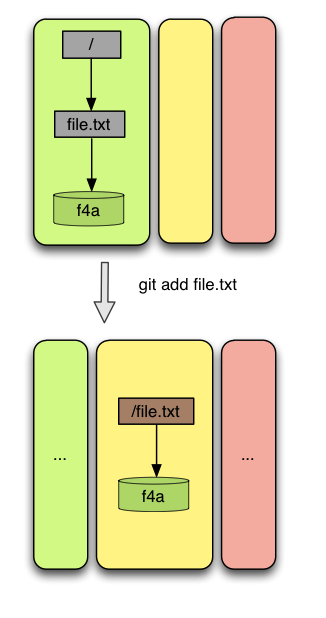
\includegraphics[width=0.8\textwidth]{images/add1.png}
      \caption{Adding a file}\label{fig:add1}
   \end{minipage}
   \begin{minipage}[b]{0.5\linewidth}
      \centering 
      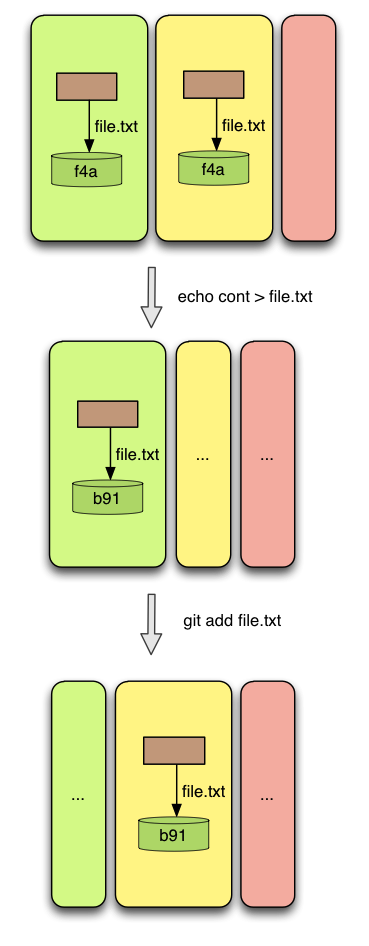
\includegraphics[width=0.9\textwidth]{images/update1.png}
      \caption{Updating a file}\label{fig:update1}
   \end{minipage}
\end{figure}

Figure \ref{fig:update1}, contains the case of updating the content of a file.
Assuming that the file is already in the index, changing its content in the 
working directory, will not change the content in the index. We need to 
explicitly add the file with the new content in the index. \\ 

Now lets loot at the remove operation. Figures \ref{fig:remove1},\ref{fig:remove2} 
show a simple case of
removing a file from the index. As the reader can see the file will be
removed from the index, but also from the working directory. 
There are no changes on the repository.


\begin{figure}[tp]
   \centering
   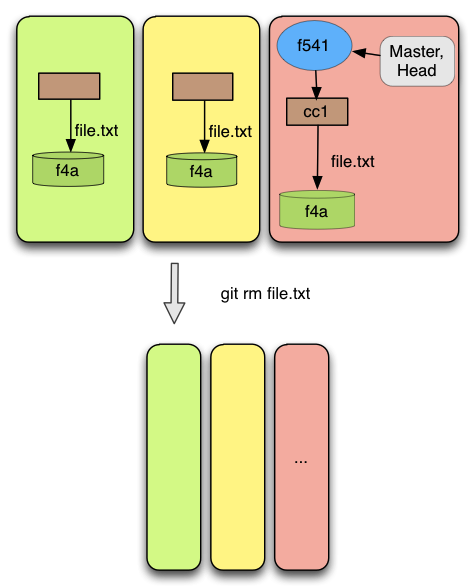
\includegraphics[width=0.6\textwidth]{images/remove1.png}
   \caption{Removing a file}\label{fig:remove1}
\end{figure}

\begin{figure}[tp]
   \centering
   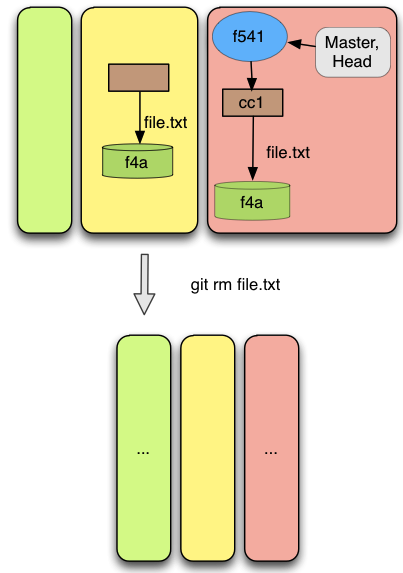
\includegraphics[width=0.6\textwidth]{images/remove2.png}
   \caption{Removing a file (alternative)}\label{fig:remove2}
\end{figure}



\subsection{Commit}
The commit operation takes the current index and builds a commit
object. Basically it takes the files from the index, builds a
structure using trees and blobs objects and creates a new commit
object pointing to the tree that corresponds to the project's root
directory. This commit object will have as parent the current commit,
the commit pointed by the branch indicated in the HEAD.
When the first commit is created, a branch called "master" will be created
and it will be marked as the current branch, or in other words, it
will be indicated by HEAD. Also, the first commit of the repository
is called a Root Commit, because it has no parents.

\subsubsection{Pre requisites}
There are three pre-conditions that are required to perform this
operation:
\begin{itemize}
   \item The index is not empty;
   \item The commit object that will be created is different from the
   current commit;
   \item There are not unmerged files.
\end{itemize}
The first pre-condition is obvious, because if we do not have files in
the index, there is anything to commit.\\

The second condition says basically
that we cannot have two commits objects pointing to the same
tree object in a row, or in other words, if we have the same files and
the same content in the index and in the current commit, a commit
operation cannot be performed. \\

The last condition just says that it is not possible to perform a
commit, if there are unmerged files in index. As we have said before,
we will speak about this later.

\subsubsection{Result}
The result of performing a commit can be different if it is the first
commit or if there are already some commit in th repository. 
We start by exposing the observed result when the first commit is
being performed and then we show the case when there are already some
commit in the repository. In the end we show some properties that are
observed in both cases.\\

The first commit object that is being created is a commit with no
parent. It means that it does not have a parent. There cannot be branches
at this moment, because they cannot point to any commit, as there are none to be
pointed, so a new branch called "master" is created. This branch is going to be pointing to 
the commit that has been created. Also the HEAD, that previously was 
not defined will identify this "master" branch.\\

When there are already some commit in the repository, then it is
guaranteed that there are at least one branch and the HEAD is
identifying some existing branch. The branch that is identified by the
HEAD, is pointing now to the commit created. This commit have now as
parent the previous commit (the commit pointed by the branch
identified by the HEAD), unless it is a result from a merge. In this
case the commit must have two parents. The previous commit and the
branch that is being merged.\\

The common properties that are observed are that all the files and
content that were in the index, are now in the current commit with the
structure from the file system. For this new blobs and trees were
probably created. The index keeps exactly the same content.

\subsubsection{Examples}

The figure \ref{fig:commit1} shows as typical process where there are added
some files to the index and then is done a commit. As can be seen the new commit
reflects, the structure of the working directory at that point. 
The interesting thing here is that, because the two files
have the same content, they will share the same
Blob. This is a case where \emph{git} shows its efficiency. \\
Figure \ref{fig:commit2} has an example of a commit operation, where in 
already exists a commit object in the repository. This figure is 
interesting because it shows what changes are done in the repository when a
new (not RootCommit) is done. The new commit points to the previous commit, and
the branch and HEAD point to the new commit. As expected the new commit reflects
the working directory structure at the point of commit.\\
Figure \ref{fig:commit_pre} is just a concrete example of the 2nd pre requisite
referred above. \\

\begin{figure}[!t]
   \centering
   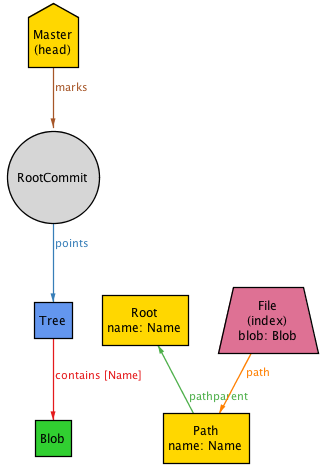
\includegraphics[width=0.8\textwidth]{images/commit1.png}
   \caption{Doing a commit}\label{fig:commit1}
\end{figure}
\begin{figure}[!t]
   \centering
   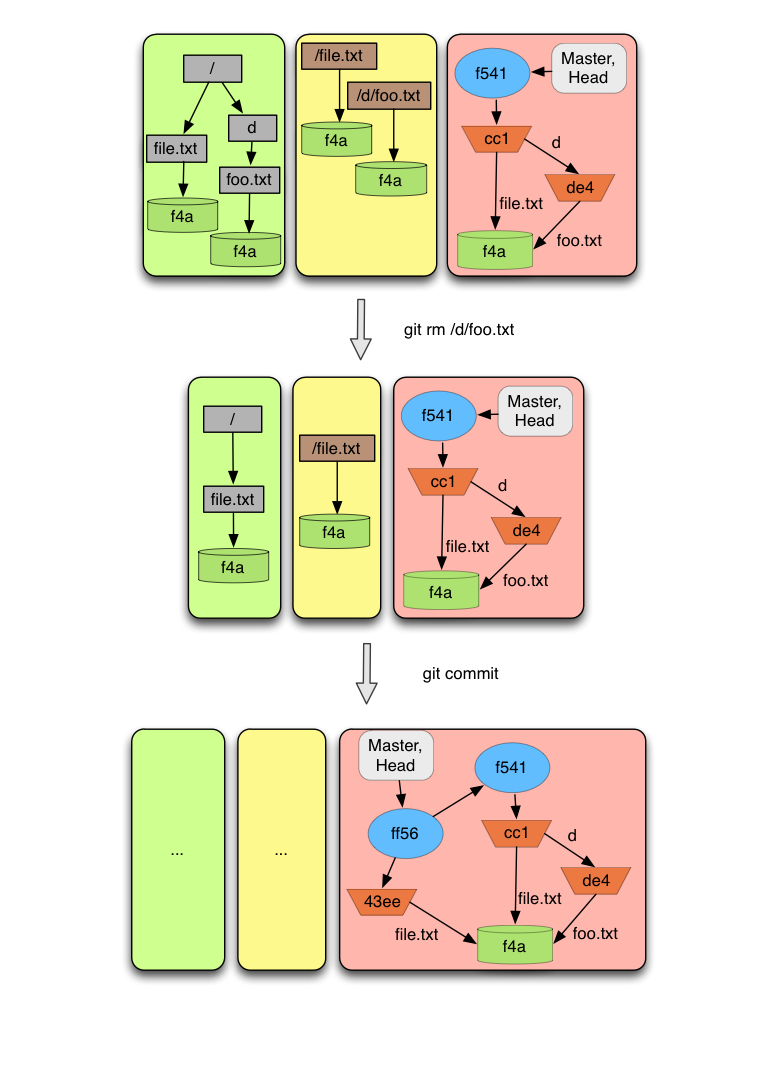
\includegraphics[width=0.8\textwidth]{images/commit2.png}
   \caption{Doing a second commit}\label{fig:commit2}
\end{figure}

\begin{figure}[!t]
   \centering
   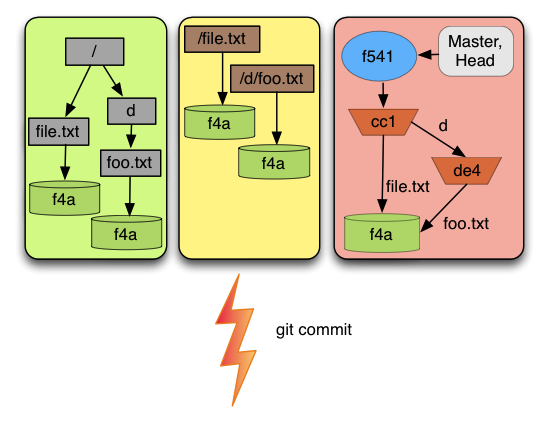
\includegraphics[width=0.6\textwidth]{images/commit_pre.png}
   \caption{This commit can't be done in \emph{git}}\label{fig:commit_pre}
\end{figure}

\subsection{Branch Create and Branch Remove}
Branches in \emph{git} are very efficient. This happens because a
branch in \emph{git} is just a pointer to a commit. So, when a branch
is created or removed there is only a new pointer created or a
pointer that is removed. As we will see later, there are some
restrictions when removing branches. When we are referring to
creating or removing a branch, we mean the operations
\emph{git branch} and \emph{git branch -d}.

\subsubsection{Pre requisites}
When creating a branch there are only two restrictions:
\begin{itemize}
   \item Some commit must exist, and consequently the HEAD reference must point
   to some commit;
   \item There is not any branch with the same name.
\end{itemize}
The second pre-condition is kind of obvious. We cannot create a branch
with the same same name as one already in the repository, otherwise we
would have conflicts. The pre-conditions that could bring some doubts
is the first one. \emph{Git} does not allow the creation of branches
before the first commit is done. When the first commit is done, a
branch called "master" is created and after that it is possible to
create as many branches as the user wishes.\\

When removing a branch there are also some restrictions:
\begin{itemize}
   \item The branch exists;
   \item The HEAD is not identifying the branch;
   \item The commit pointed by the branch is accessible from the
   current commit (the commit pointed by the branch identified by the
   HEAD).
\end{itemize}

The first pre-conditions says that it is only possible to remove a
branch if it exists. The second says, that the branch being removed is
not the one identified by HEAD, otherwise the HEAD would be point from
now on to some branch that does not exists anymore. Thus, there would
not exist a current commit. The last pre-conditions exists to check
the user does not deletes a branch that is not yet merged with the
current branch, or in other words, the user does not delete a branch
that is not accessible from the current commit, through the parent relation. 
If this pre-condition did not exist it would be possible to loose the
commit pointed by the branch, as well as, some commits from the parent
relation.


\subsubsection{Result}
The result of performing this operations are expected. When creating a
branch, the result is a new branching pointing to the same commit as
the branch identified by the HEAD. When removing a branch, the result
is that the branch removed does not exists anymore.

\subsubsection{Examples}
The changes that happen when creating a branch are minimal. The only thing
changing is the appearance of a new branch pointing to the current commit, as
figure \ref{fig:branch} demonstrates. \\ 
The removal of a branch is also minimal. The only thing changing is that the 
branch referred must be deleted. If in \ref{fig:branch} we view 
the grey arrow as pointing up, instead
pointing down, we automatically view the process of deleting a branch. \\ 
About the branch removal pre condition, this case
is legit because the current commit achieves (it is the same) the
commit pointed by the branch deleted. Even if 'Foo' pointed to any other commit, 
it could be still deleted, as all commits in this figure
are achieved by the current commit. \\

\begin{figure}[!t]
   \centering
   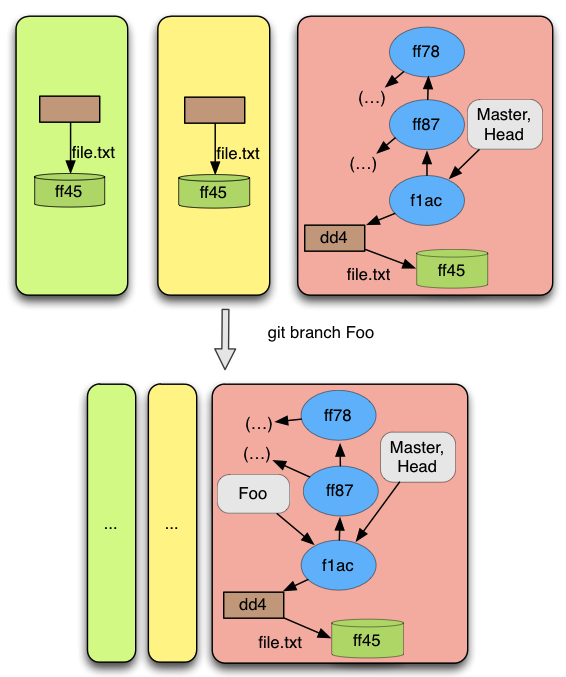
\includegraphics[width=0.6\textwidth]{images/branch.png}
   \caption{Creating a branch}\label{fig:branch}
\end{figure}

\subsection{Checkout}
The checkout operations is used to update the working directory and
index with a set of files from a commit. In this project, we have
explored only the case the checkout operation is used with a branch.
In this case, all the files from the commit pointed by the branch are
exported to the working directory and index. This was the most
difficult operation to explore, because it behaves in a non intuitive
way. We will try to explain it and in the examples we show you a
sequence of operations that causes the \emph{git} to loose
information. This is a proof of the complexity of this operation.

\subsubsection{Pre requisites}
As we have said before, this operation is not intuitive. In our
opinion this operation should have as pre-condition something like
"Everything that is in index should be committed". Instead \emph{git}
tries to relax this pre-condition and we have the following:
\begin{itemize}
   \item The branch we are checking out, exists;
   \item Everything that is in the index has to be in the current commit with the
      same content, except if:
      \begin{enumerate}
         \item The content of a file is the same in the
         current and destination commit (warning is thrown)
         \item Exists a file in the index, and that file does not exists
         neither in the current nor in the destination commit (warning is thrown)
         \item Content of the file in the index is the same as in the
         destination commit (no warning is thrown)
      \end{enumerate}
\end{itemize}

About the pre-condition there are not much to say. If we want to
checkout a branch, the branch should exist.\\

The problem here is the second pre-condition. There are a lot of
exceptions when a file is not in the current commit with the same
content. To simplify the exposition of this pre-condition, lets assume
we have a file f, which is not in current commit, or at least it is not
with the same content. All other files from index are in the current commit, with
the same content. Relatively to f, if at least one of the exceptions enumerated above
is satisfied, then the checkout operation will proceed. Now lets
analyse each one of the exceptions. The first says that, f can 
be in the commit we are checking out with the same content. So, even
if f is not commit, but it is in the commit we are checking out, git
will proceed with the operation. The exception marked as 2, says that
f does not exists neither in the current commit nor in the commit we
are checking out. It means that if f has just been created and a
checkout operation is performed then if the file does not exists in
the commit being checked out, the operation will proceed. The last
exception says that if there exists a file with the same path and the
same content in the commit being checked out, then the operation will
proceed. In this last case does not warns the user.

\subsubsection{Result}
As we have said before, in this manual we have
concentrated our efforts in the index and repository, simplifying as
most as possible the working directory. So, we will just explain what
happens with the index after a checkout operation is performed. We do
not make any description about the files that are in the working directory
but not in index.\\

The first thing the reader should know is that the
HEAD, after a checkout is performed, identifies the branch which was
checked out.\\

There is one more alteration. The index when a checkout is performed
has to be updated to reflect the operation. The result of it is not intuitive. To
understand it lets assume that the checkout operation has not yet been 
performed. Consider three relations from file to content. 
\begin{itemize}
   \item $CA$: Files from the current commit and their
   respective content;
   \item $IA$: Files from index and respective content;
   \item $CB$: Files from the commit we are trying to checkout
   and their respective content.
\end{itemize}
After understanding this three relations it is simpler to understand
what happens with the index. Lets also assume that $(IA-CA)$ is a relation that
contains the files from $IA$ which are not in $CA$ with the same content.
It mean that $(IA-CA)$ will contain the new files and the modified files relatively to
the last commit. Now, consider $CB ++ (IA-CA)$ as being all the files
from $CB$, but if the files are in $(IA-CA)$, they will keep the
content from $(IA-CA)$. If when comparing the index with the current
commit it contains only new files and modified files (not deleted
files) then it is all. $INDEX = CB ++ (IA-CA)$. When the index
contains removed files, or in other words, files that are in $CA$ but are not in
$IA$ ($CA-IA$ is not empty), then case the file that is marked as removed exists
in CB it will be marked as removed, otherwise the removed information is
ignored. So, the result of performing a checkout is: $INDEX = (CB ++
(IA-CA)) - (CA-IA)$. All files from $CB$ are overwritten by the files
that are in the index but not in CA and from the result of this, the
files that are marked as removed will not be in index.

\subsubsection{Examples}
As referred above checkout behaves in a non-intuitive way. We recommend that
every time, a checkout is done, all things must be previously committed, or else
we risk ourselves to pass things that we don't want to other branches, or even
loose information. \\
Thus, the example shown in figure \ref{fig:checkout}, contains the case where
all content in the index and working directory are committed (the safe case).
When doing the checkout we can see in the figure 
that the repository and index change to reflect the branch checked out, more
concretely the most recent commit of the branch. But
also, the commit referred will now be pointed by the HEAD reference. So, all new
changes done will belong to the branch checked out. \\


\begin{figure}[!t]
   \centering
   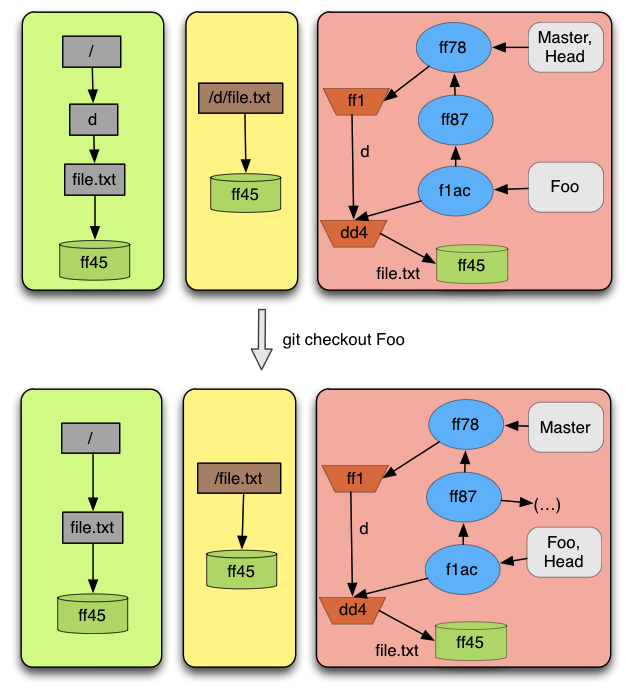
\includegraphics[width=0.6\textwidth]{images/checkout.png}
   \caption{A simple checkout}\label{fig:checkout}
\end{figure}

\subsection{Merge}

The merge operation is one the of most important operation on \emph{git}. It
consists on trying to combine information from two commits. Resulting of that
is a new commit with information from both commits, however there are some cases
where this will not always be true. A commit information can take precedence
over another, thus there is no need for a new commit. Also, the process of
joining information cannot be done, because it is not certain which
correspondent data in both commits should take precedence (merge conflict).\\

When a 'git merge <branch>' is done, \emph{git} will pick both involving
commits (the current commit, and the commit pointed by the branch referred)
and try to merge them into a new commit that must belong to the current branch.
\\
As already said, a merge conflict can happen, and if it occurs \emph{git} leaves
to the user the process of resolving the conflicts. When that process is done,
the user can notify \emph{git} by doing a 'git commit', and a new merge commit 
will be made, where its parents will be both commits trying to be merged. \\
\emph{Git} tries to be the most autonomous possible when merging, thus it has
three types of merge

\begin{itemize}
\item A fast-forward merge (figure \ref{fig:fast_forward}). 
Happens when the non current commit, can achieve the current commit by the 
parent relation. If that happens, then the non current commit is more recent
than the current commit, so the merge commit would be equal to the non current
commit. Because \emph{Git} tries to be efficient a merge is not made. But, the
HEAD will point to the newest commit. 

\item A 3-way merge (figure \ref{fig:3mergecase}). 
Happens when a fast-forward is not possible, but, both commits have a common
ancestor. \emph{Git} will use the common ancestor to minimize potential
merge conflicts.

\item A 2-way merge (figure \ref{fig:2mergecase}). 
Happens when both types above are not possible. In this case there are no
common ancestor, thus will it be more likely that conflicts appears.

\end{itemize}

\subsubsection{Pre requisites}
The merge operation, as all other operations has some pre conditions that
must be satisfied in order to be possible to do it. As in the checkout,
\emph{git} let's the user do merges without all information in the index 
being committed. However,again, it is recommended that no information is 
left uncommitted :

\begin{itemize}
\item A merge can't be made, if the current commit is more recent than the
other. As the current commits takes precedence, no new changes will exist. 
Thus, the merge is not necessary.
\item If \emph{git} can't do the merge automatically because of conflicts,
the user must resolve all those conflicts, before doing another merge.

\item When it is the case of a fast-forward merge, the index can't have 
uncommitted files that would be changed by the resulting merge.

\item In the case of a 2-way or 3-way merge operation there simply 
can not be uncommitted files.
\end{itemize}

\subsubsection{Result}
As already said when doing a merge, one of three things can happen. A 
fast-forward, a successful merge or a partially done merge:

\begin{itemize}
\item If it is the case of a fast-forward merge. The index and the working directory
will contain the information of the newest commit. Also, they will contain all 
information prior to the merge that was uncommitted, as long as that it brings
no conflicts to it. Of course, the current branch and HEAD will point to the
newest commit.

\item When a successful merge happens, the index will reflect the new commit,
and the working directory will contain the information of the commit. Here,
doesn't exist the question of uncommitted changes, as \emph{git} forbids that
to happen. In the repository a new commit will appear that has the combined
changes of the two (possibly three) commits involved in the merge. That new
commit will have as parents those two commits, and will be pointed the current
branch and the HEAD.

\item If when doing a merge, a conflict appears that \emph{git} can't resolve,
it will say that the automatic merge failed, and that the manual merge will
begin, in other words it leaves to the user the work of resolving the conflicts
that \emph{git} couldn't solve. At that moment, the index and working directory
will contain all the information that was merged. For all the files unmerged, they
will also be maintained in the index and the working directory, but in a
state where we can see what differs in them, when they belong to a commit or to
the other. Finally, \emph{git} will mark some fields in the repository, so that
when the user does the next commit, it will be the son of both parents
involved in the commit, where it will be pointed by the current branch and HEAD.
When this new commit is done, the merge process is over.

\end{itemize}

\subsubsection{Examples}

As usual the next figures will show some concrete examples of what happens
in \emph{git} when a merge is done, we don't involve here cases of 
uncommitted changes, as we don't recommend to do that and 
things would turn much more tricky to understand and much less intuitive. \\

Figure \ref{fig:ffmerge1} is a simple case of a merge operation. It shows
that the Master branch and HEAD point to a commit that is achievable by the
commit pointed by 'Foo', so this is a case eligible for a fast-forward commit.
We can see that the result is that the working directory and index will be
updated accordingly to the commit now pointed by 'Foo' Master and HEAD. As
known any untracked file will not be changed. \\

Figure \ref{fig:ffmergepre} shows a concrete example of state in the repository
where it is not possible to do a merge. As the commit pointed by HEAD and Master
can achieve the commit pointed by 'Foo', thus the current commit taking
precedence over any data than the other commit could have. \\

The two last figures \ref{fig:merge2way} and \ref{fig:merge3way} demonstrates 
the difference between a 2-way and a 3-way merge commit. When in the 2-way there
are conflicts to resolve, in the 3-way the conflicts are resolved by looking to
the common ancestor. Because the 3-way merge was automatic, a new commit was
created that represent the merged information. Also, the working directory and
index were updated accordingly. In the 2-way the user had to resolve the
conflict by adding new content to the unmerged file and adding it to the index.
Finally, when 'git commit' was called a new merge commit was created and 
the merge process successfully finished. In this case the index and working 
directory were updated just before \emph{git} leaved to the user the merging
process. \\

\begin{figure}[!t]
   \centering
   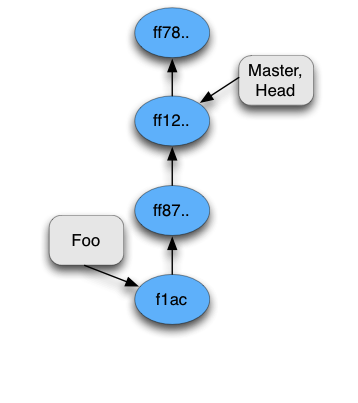
\includegraphics[width=0.5\textwidth]{images/fast_forward.png}
   \caption{A fast-forward case}\label{fig:fast_forward}
\end{figure}

\begin{figure}[!t]
   \centering
   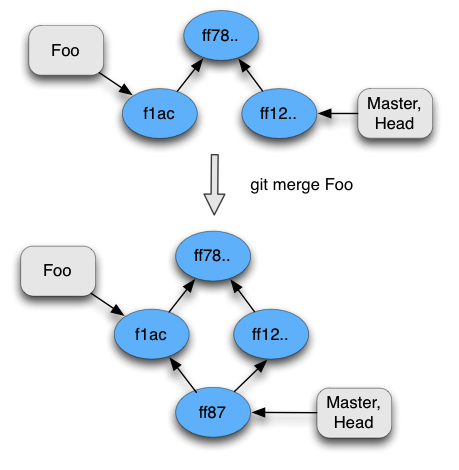
\includegraphics[width=0.6\textwidth]{images/3merge.png}
   \caption{A 3-way merge case}\label{fig:3mergecase}
\end{figure}
\begin{figure}[!t]
   \centering
   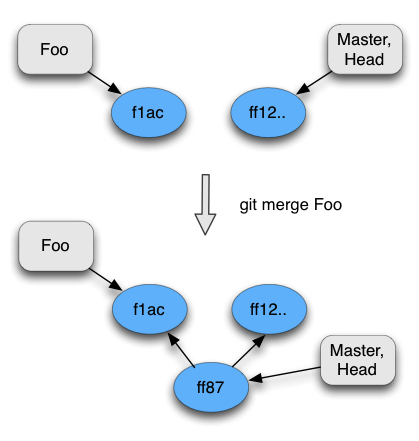
\includegraphics[width=0.6\textwidth]{images/2merge.png}
   \caption{A 2-way merge case}\label{fig:2mergecase}
\end{figure}
\begin{figure}[!t]
   \centering
   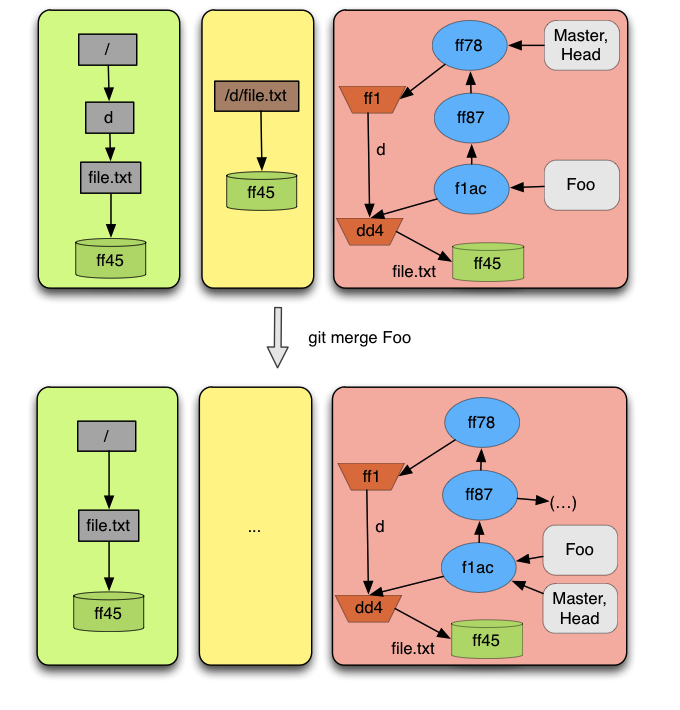
\includegraphics[width=0.6\textwidth]{images/fast_forward_merge1.png}
   \caption{A fast-forward merge case}\label{fig:ffmerge1}
\end{figure}

\begin{figure}[!t]
   \centering
   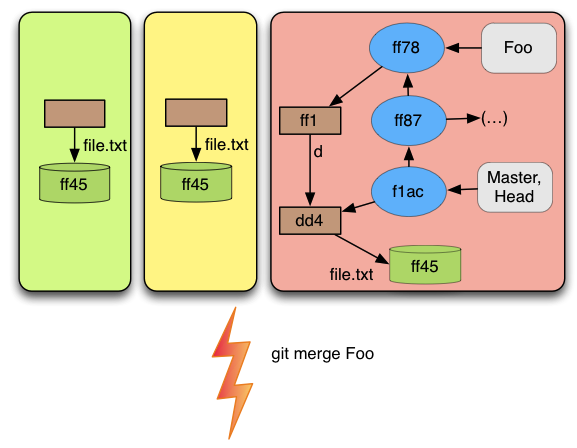
\includegraphics[width=0.6\textwidth]{images/fast_forward_merge_pre.png}
   \caption{A fast-forward case that can't be done in
   \emph{git}}\label{fig:ffmergepre}
\end{figure}

\begin{figure}[!t]
   \centering
   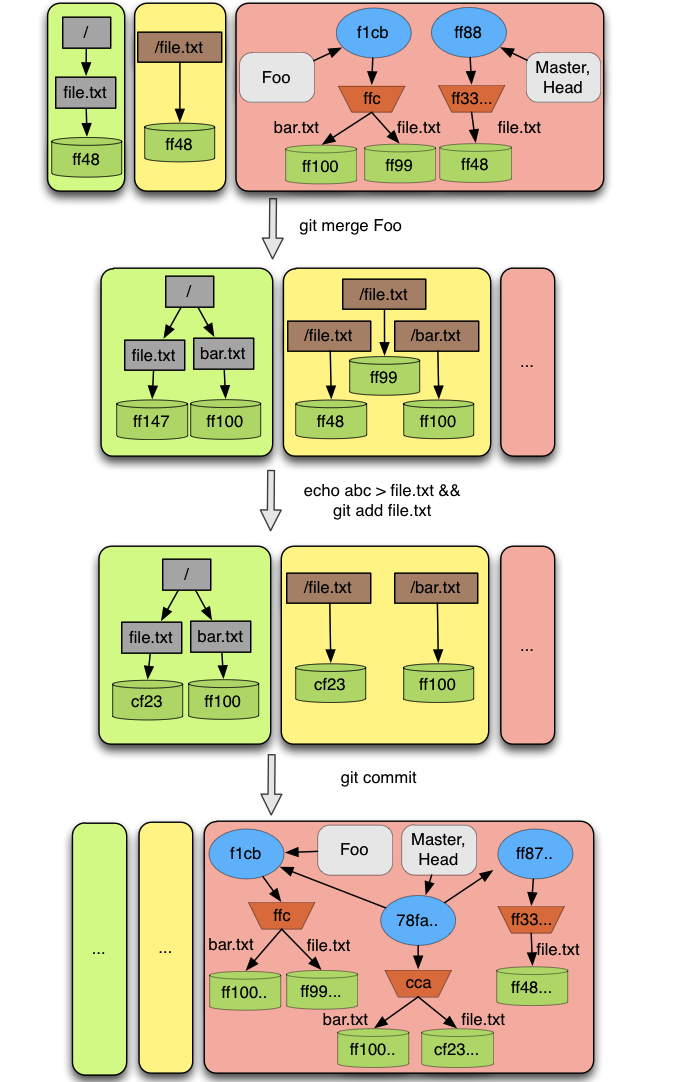
\includegraphics[width=0.7\textwidth]{images/merge2way}
   \caption{A typical 2-way merge}\label{fig:merge2way}
\end{figure}
\begin{figure}[!t]
   \centering
   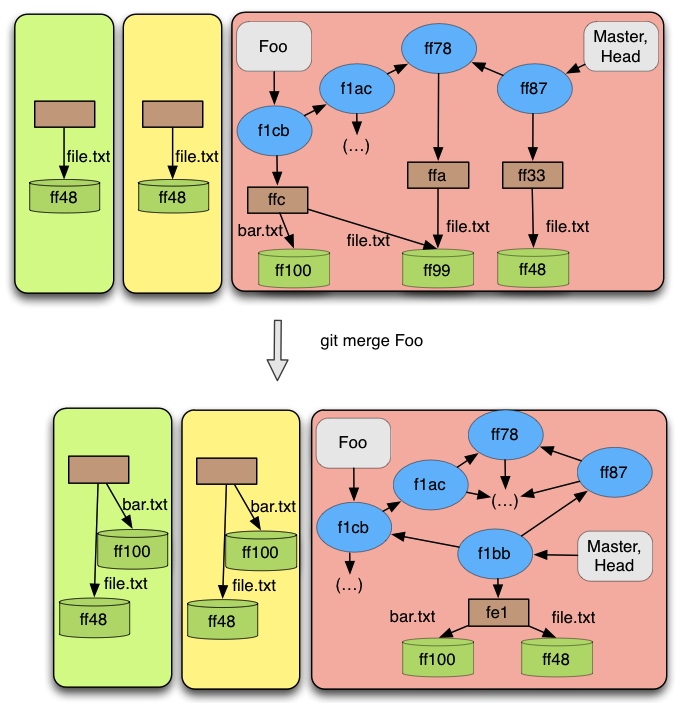
\includegraphics[width=0.7\textwidth]{images/merge3way}
   \caption{A typical 3-way merge}\label{fig:merge3way}
\end{figure}

\subsubsection{Git Pull and Git Push}

When working with remote repositories, these two operations will be vastly
used. They are in fact, a sequence of operations, and are used to get content
from a remote repository or to upload local content to the remote repository.
\\
If a 'git pull' is done, the branch from the remote repository will be fetched,
and the local branch and the remote (now, also local) branch will be merged. So
expect this operation to behave exactly like a merge operation and consequently
all that was referred in the merge applies also here. \\
If a 'git push' is done, the local branch will be uploaded to the remote 
repository and will be merged there. \\
In Push there is an important restriction. A 'git push' 
can only be done when the resulting merge is a
fast-forward. This happens because, there is no one on the other side to resolve the 
merge conflicts, and thus \emph{git} must guarantee what no conflicts happen. 
